SyVOLT has a number of unique features, outlined below.

\subsection{Graphical Modelling of Model Transformation Contracts}

SyVOLT proves pre-/post-condition contracts hold for a model transformation.
Such contracts establish relations between patterns occurring in input and output
models of a model transformation. If a contract holds, then a formal guarantee
exists that whenever an input model contains the pattern specified in the
pre-condition of the contract, the output model contains the pattern specified
in the post-condition part of the contract and any traceability relations
between the two. Due to the graph-like structure of the pre and post conditions
of contracts, the visual representation of the contract in SyVolt editor allows
the user to quickly build and intuitively understand their meaning.
%If a textual (logical or mathematical) editor where to be used, the user would
%need an extra system of identifiers to correctly prescribe the associations
% between pre and post-condition elements whereas in the visual representation, the user graphically builds the associations between those elements.
%\levi{Claudio, I don't understand this sentence}
%\cgg{Please tell me now if you can understand it.}

%The visual representation of a contract has all the necessary information to
% derive the correct logical expression to be used by the internal SyVolt prover.

\subsection{Push-Button Proofs}
\label{sec:push_button_proofs}
SyVOLT is a verification tool that provides formal guarantees of correctness of
a model transformation. The proving process is fully automatic and
the all formal details are completely hidden from the user, who only needs to specify a
set of contracts for the transformation being verified. Once the transformation and the
contracts of interest are created, one command will start the property proving
process. This process will automatically create all required artifacts (as
detailed in the following section), run the process, and then provide the
results to the user within the Eclipse environment, as seen in
Figure~\ref{fig:output}. This allows the user to continually stay within the
Eclipse environment, which is where he develops the contracts and the model
transformations.

\subsection{Based on Symbolic Execution}

Our technique shares its principles with symbolic execution, a classic method to
verify code. The underlying idea entails building a finite representation of the
(infinite) set of computations that can be built by a model transformation
specification. In this context, each symbolic execution (also called
\emph{path condition}) consists of a combination of a subset of the rules of the
model transformation being verified in a way that it represents the execution of the the model transformation over any input
model those rules match on. Then, properties of interest can be proved on the
set of generated path conditions and extrapolated to the infinite set of the
model transformation's potential computations.

% Our model transformation verification technique relies on models as the
% means to internally represent both symbolic executions and contracts. SyVOLT
% then reasons over these graphs to build a proof that contracts hold or do not
% hold.

% Note that by using a typed graph representation, our technique can prove
% contracts that include constraints on the structure and the attributes of the
% input and output models. 

% \levi{keep the text from here on?} An example of this would be in the
% Families-To-Persons transformation from the ATL zoo [CITE]. In this transformation, the name for a person in the
% output graph is a concatenation of two strings \cgg{instead of ''strings``,
% should be ''attributes``} from elements in the input graph. Our contract prover
% can prove that this concatenation will be valid in all cases.

\begin{figure}
\centering
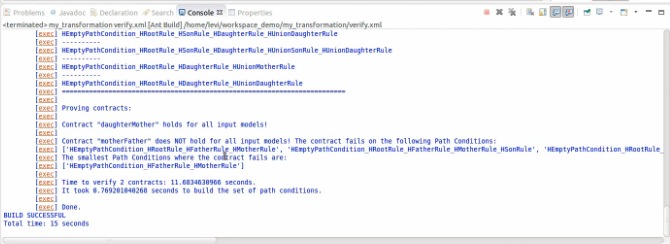
\includegraphics[width=0.5\textwidth]{figures/output}
\caption{The results of the contract prover}
\label{fig:output}
\end{figure}

\subsection{Input Independence and Exhaustiveness} 

Our technique is exhaustive, in the sense that whenever a contract holds, it
will hold for all possible input models to a transformation. This is possible
because SyVOLT operates on specifications of outplace model transformations
where unbounded loops and model element deletions are not allowed. SyVOLT thus proves
contracts in an input-independent manner, relying only on the specification of the
transformation. The soundness and completeness of our technique is described
in~\cite{Lucio2014}.

\subsection{Proving Contracts about ATL Model Transformations}
The Atlas Transformation Language (ATL)~\cite{atlTool} is commonly-used in both
industry and academia applications. In order to extend our approach into these domains, we
have developed a higher-order transformation that is able to automatically
transform declarative ATL transformations into our transformation language
DSLTrans~\cite{Oakes}. This allows the user to also prove contracts on
ATL transformations.

\subsection{Scalability and Speed}

We have some evidence that SyVOLT scales to transformations of practical
interest. This has been empirically shown by applying it to DSLTrans
transformations with up to over 60 rules, and ATL transformations with up to 13
rules~\cite{Oakes}. From our own experience with DSLTrans, the size of a
DSLTrans transformations varies widely, with the average size ranging from 10 up
to 50 rules. The average size of an ATL transformation is around 20 rules. [cite
Manuel's paper, should we keep this?] \cgg{The problem is that there is not enough infor about those 20 rules. Are they imperative? Do they use imperative helpers? How many rules are generated when those transformations are translated to DSLTrans?}.
Even though our technique is exhaustive, our approach takes relatively short
amounts of time to prove contracts. For example, our experiments with industrial
transformations~\cite{Oakes} show that contracts can be verified within a few
minutes. In Gehan Selim's PhD thesis~\cite{Selim2015}
further evidence of SyVOLT's speed is given when verifying a relatively large
model transformation for giving semantics to the UML-RT language in terms of
the Kiltera process language~\cite{PosseDingel2014}. SyVOLT's symbolic execution
engine is fully homegrown~\cite{LucioVang} and does not depend on third-party
solvers \cgg{This sentence and the next one are part of the "how". Hence, they should be in the Architecture section. The highlight here is the speed and not how that performance was achieved. Correct?}. Although this has implied a large effort to build the codebase, it has
also allowed us to have the required control over the code to iteratively
optimize the engine for both space and time economy. \cite{Selim2014}
demonstrates that our prover is substantially faster than similar approaches based on SAT solvers.


\subsection{Production of Counter-Examples}

When a contract is proved to be violated by a given model transformation, it is
useful to also provide an input model - called a \emph{counter-example} - so
that the user can execute the model transformation with that input and verify
that indeed it violates the contract. The counter-example produced by SyVOLT
consists of a set of rules involved used to build a particular symbolic
execution where the contract does not hold. In this sense, a counter-example
describes a family of input models that violates the contract. By examining the
counter-example, the user can determine which rule(s) produce the error in the
transformation and correct it.
%  This means that any input model that belongs to the family of the
% counter-example - i.e., fits the description given by the contract proving
% process - causes the model transformation to violate the contract.
% We suggest that this supports a transformation
% development method analogous to 'test-driven development'. In this method,
% development would be routinely punctuated by contract proof in order to catch
% errors early and store test cases - the counter examples produced - to be used
% in the future.


\subsection{Integration with Eclipse}

Eclipse is a popular development environment and model transformation
tools such as ATL~\cite{atlTool}, DSLTrans~\cite{Barroca2011} and
EGL~\cite{eglTool} are integrated with the Eclipse Modeling Framework
(EMF)~\cite{emfTool}. To take advantage of this ecosystem, SyVOLT integrates
with EMF too. In the EMF, models can be represented in a multitude of syntaxes, from
graphical to textual, and this makes the interaction with SyVOLT easier since the modeler
can use the model editor that he/she finds most convenient.
%Internally, SyVOLT uses the Himesis format~\cite{Provost2006} to represent
% models.

%\subsection{Model Driven Developed GUI\levi{this text is subsumed by section
%III a)}}
%\label{sec:mdd_gui}

%To take advantage of the productivity promised by MDD, we used a language
% called Eugenia[CITE] to develop the SyVolt contract editor shown in
%Figure~\ref{fig:eclipse_frontend}.
%With this approach, the SyVolt editor was developed in about 4 man-hours.

\begin{figure}
\centering
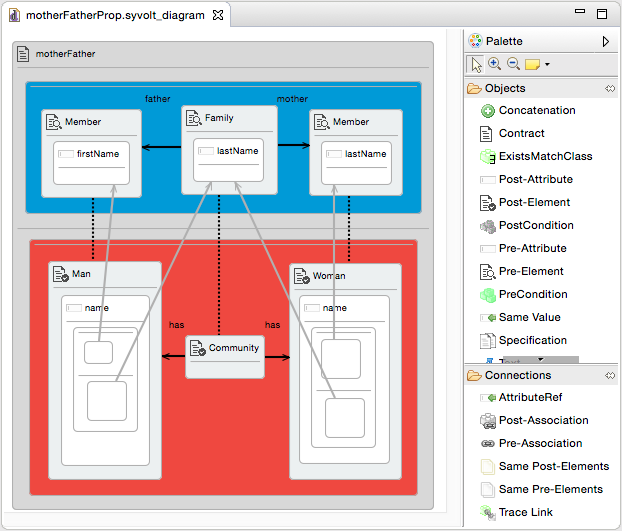
\includegraphics[width=0.5\textwidth]{figures/eclipse_frontend}
\caption{The transformation editor within Eclipse}
\label{fig:eclipse_frontend}
\end{figure}




 